% This file is based on the "sig-alternate.tex" V1.9 April 2009
% This file should be compiled with V2.4 of "sig-alternate.cls" April 2009

\documentclass{sig-alternate}

\usepackage[english]{babel}															% English language/hyphenation
\usepackage{url}

\usepackage{etoolbox}
\makeatletter
\patchcmd{\maketitle}{\@copyrightspace}{}{}{}
\makeatother

%%% Maketitle metadata
\newcommand{\horrule}[1]{\rule{\linewidth}{#1}} 	% Horizontal rule

\title{
		\vspace{-0.4in} 	
		\normalfont \normalsize \textsc{Rochester Institute Of Technology} \\ [15pt]
		\today\\
		\horrule{0.5pt} \\[0.4cm]
		\huge Holographic Pong \\
		\horrule{0.5pt} \\[0.4cm]
		\normalsize\vspace{-0.5in}
}
\author{
		\normalfont 
        Vasudev Prasad, Piter Garcia, Jorge 
        \\[6pt]\normalsize
}

%%% Begin document
\begin{document}
\maketitle

\begin{abstract}

Holography is a technique used to display objects or scenes in three dimensions. These 3-dimensional images, or holograms, can be seen with the unassisted eye and they are very similar to how humans see the actual environment that surrounds them. Unfortunately, this technique has not been very successful, principally due to the computational complexity of calculating diffraction patterns in real time and poor quality of the resultant images. In our project, our goal is to overcome these problems to enable a high quality and real time holographic projection of a pong game that we are developing. In order to approach our goal, we are making use of a holographic stereo-graphic technique and a acrylic material as the medium to demonstrate a holographic display of our pong game. A projector is used to project the holographic image or multicolored holographic 3D images produced by our code implementation. 

\end{abstract}

\section{Overview}
\label{overview}

	The logical structure of our project is composed of three main phases, which better describe the milestones achieved throughout our project development. These phases are classified as Design, Architecture and Implementation. Each phase explains in detail the main steps taken to model and structure a 3D Pong game with a Holography Display Case built to meet the project specifications. In order to better organize our documentation we have divided each phase into two main sections that contain a summary of the work process done in our project. These two sections are Software and Hardware, and their development can be described in three main divisions that took place in order to build our holographic 3D Pong game. 
	\newline
	
	In the Software section, we will elaborate how we designed the 3D Pong game and present the techniques that form part of the concept used to create our 3D game structure. In the structure section, we will explain the tools and techniques planed and used to make the logical structure of our game possible. Lastly, in the performance section, we show how to combine both the design and structure to successfully implement our 3D game.
	\newline
	
	In the Hardware section, we will focus only on the tools needed to project our 3D Pong game in a holographic manner. In the design section, we will give an example of the structure designed and the reasons of its design. In the structure section, we will mention and describe the tools used to create the frame to hold and project our 3D Pong game in a real environment.  In the performance section, we will show and explain the performance while building the hardware by modeling our hardware according to the techniques and tools implemented. 
	\newline
	 
	Finally, we will explain how to implement the software and hardware we built for our project. The deliveries of our project will be discussed in the current work section, and in the future work section we will mention the issues that we had throughout the development of our project as well as the techniques and tools that may improve the implementation of our project.  
	\newline
	
\section{Design}
\label{design considerations}
	In this project, the operational process of our design meets the objective of a high quality development which responds to 3D games in real time holographic projection. The focus of this step is the development of an acceptable functional solution to the requirements of our project with an exterior design solution that is compatible with our 3D Pong game interface and our goal as a whole. The progress sets of our design were formally modified, implemented, and reviewed by our group as they were issued at the completion of our schematic design, design development, and during the development of our 3D Pong game. A successful design development was needed in order to coordinate the software and hardware project architecture to meet our goal, as these are important for our overall project development. In fact, our project design process typically involves the sequence of activities described below.

	{\bf \begin{enumerate}
			\item {Software} {\normalfont\newline 

				\bf{\begin{itemize}
					\item {Appearance} {\normalfont\newline 
					\begin{figure}[htb]
					 		\begin{center}
					 		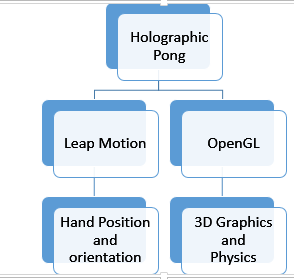
\includegraphics[width=1.2in]{sw1.png}
					 		\caption{Software Design.}
					 		\end{center}
					 		\end{figure}
					\newline
					}
		
					\item {Structure} {\normalfont\newline 
					\begin{figure}[htb]
					 		\begin{center}
					 		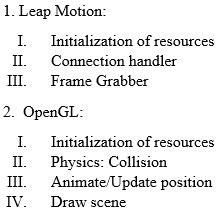
\includegraphics[width=2.0in]{sw2.png}
					 		\caption{Structure Design.}
					 		\end{center}
					 		\end{figure}
					\newline  
					} 
		
					\item {Performance} {\normalfont\newline 
						For our game, the performance needs to be real-time which we are aiming for this project. The Leap device is able to detect the hand and other point-able objects in real-time because of which we can move the paddles without any lag. The game has 3 objects in total which we imagine will be light on the physics function which checks for collision and the resultant vector. 
					\newline
					}	
			\end{itemize}}}
	\end{enumerate}}
	
	{\bf \begin{enumerate}
			\item {Hardware} {\normalfont\newline 
				We have built a holography display case by using reflecting methods to create a holographic image between physical and virtual space. In order to better explain the design of our holography display case, we have divided the hardware design in the following three sections.
			
				\bf{\begin{itemize}
					\item {Appearance} {\normalfont\newline 
							\begin{figure}[htb]
										 		\begin{center}
										 		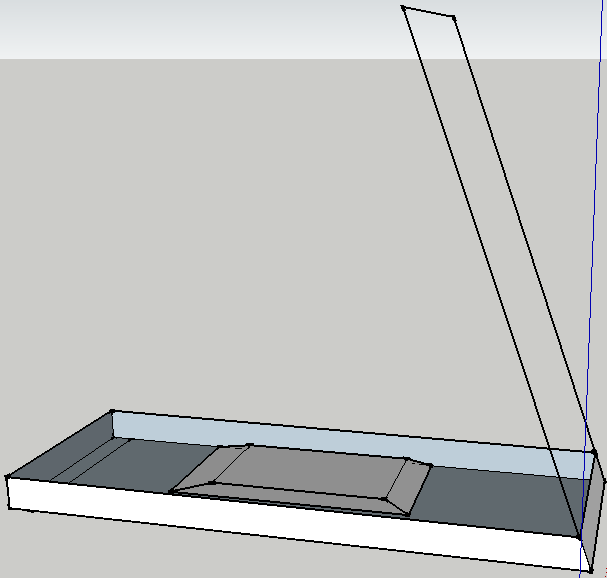
\includegraphics[width=2.0in]{p1.png}
										 		\caption{Hardware Design1.}
										 		\end{center}
										 		\end{figure}
							\begin{figure}[htb]
												 \begin{center}
										    	 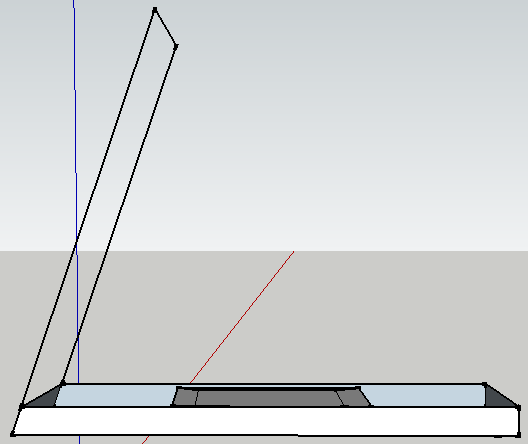
\includegraphics[width=2.0in]{p2.png}
												 \caption{Hardware Design2.}
												 \end{center}
												 \end{figure}
												 
						Figures 3 and 4, is the design we used to create our own hardware for holographic display. As you can notice in the design sketch, the base had to be of a strong material, metal perhaps, and the top is a made of crystal in order to project the image. The small object that, shown in the middle of figures 3 and 4, is the projector. This will send the 3D image of our game to the acrylic glass, which will then reflect it as it if was part of the actual real environment.
					\newline
					}
		
					\item {Structure} {\normalfont\newline
							\begin{figure}[htb]
										 		\begin{center}
										 		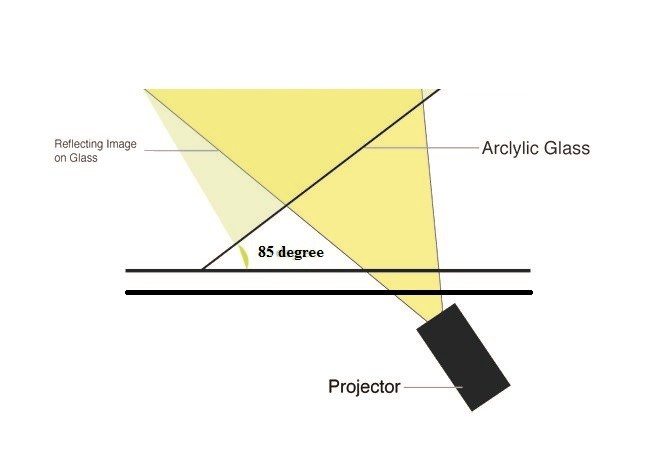
\includegraphics[width=3.0in]{p3.png}
										 		\caption{Structure Design.}
										 		\end{center}
										 		\end{figure} 
						The structure of our holography display case was based on our methodology, which we are describing below.\newline
					
						Methodology\newline
					
						In order for our holography case to project a good holographic display it is necessary to have a black background so the image can emerge from the bottom. The image will then reflect the glass, which is placed at an 85 degree angle from the base and the user. This way, the image will float up on the air like an illusion.\newline
						
						The figure 5 explains the function of the crystal. As you can see, the projector sends the image to the crystal, which is an acrylic glass, and this reflects the image at an 85 degrees. This is giving the user a real feeling about the 3D object existence.
					\newline  
					} 
		
					\item {Performance} {\normalfont\newline
						According to our design, the position of the glass would definitely influence the holographic display performance. We picked about 85 degrees because we wanted the object to look as if it was floating right in front of your eyes, without the need of having to look down. 
					\newline
					}	
			\end{itemize}}}
	\end{enumerate}}

\section{Architecture}
\label{architecture}
	It was critical to model the right architecture in order to succeed in our 3D Pong game design. The architecture system representation was essential for the description and analysis of the high level properties of our system. This essential tenet forced us to consider alternatives due to the architecture of our project. The architecture of our project specifies the overall structure of our system. This includes the projection and 3D user interaction through the Leap motion device as described below. The database contains the assignment of functionality for our designed 3D Pong game, composition of designed features, and hardware design modifications. In contrast, the hardware section includes the body of work for our module interconnection features and framework in our 3D Pong game. This serves the needs of formal models of component integration mechanisms for a holographic display. 
	 
{\bf \begin{enumerate}
			\item {Software} {\normalfont\newline 

				\bf{\begin{itemize}
					\item {Appearance} {\normalfont\newline 
							\begin{figure}[htb]
							\begin{center}
							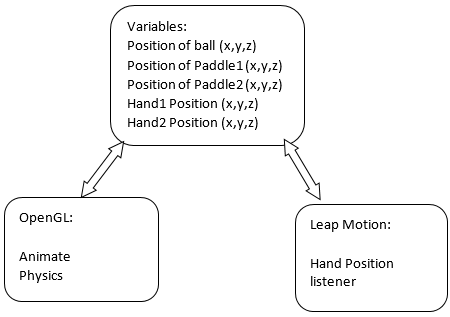
\includegraphics[width=3.0in]{sw3.png}
							\caption{Structure Design.}
							\end{center}
							\end{figure}
					\newline
					}
		
					\item {Structure} {\normalfont\newline 
						We have the variables for the position of the ball, paddles and the hand. Leap Motion has a listener class that updates the position of the hands in the palm object. We update the position of the paddles with the position of the hands as provided by the listener class. The physics function will update the variables of the position of the ball. Animate function uses these variables to translate the objects in the scene. 
					\newline  
					} 
		
					\item {Performance} {\normalfont\newline 
						As expected, the program runs in real-time. Initially, we had a problem with the update of the position of the paddles because the Leap Motion listener function was not updating the position of the paddles. We fixed this by calling the listener function before the OpenGL functions. The physics function needs work. 
					\newline
					}	
			\end{itemize}}}
	\end{enumerate}}
	
	{\bf \begin{enumerate}
			\item {Hardware} {\normalfont\newline 
				In the architecture phase of our project, the goal was to build our own holography display case as close as possible to our design. This was necessary in order to get a holographic image display for our 3D Pong game. This process can be explained as follows:

				\bf{\begin{itemize}
					\item {Appearance} {\normalfont\newline 
						\begin{figure}[htb]
							\begin{center}
							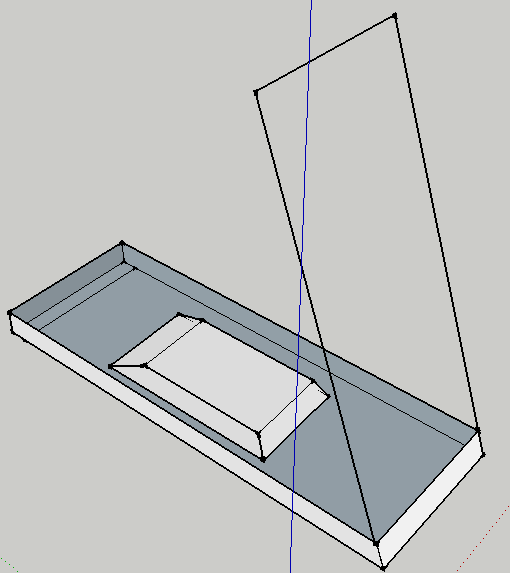
\includegraphics[width=2.0in]{p4.png}
							\caption{Structure Design.}
							\end{center}
							\end{figure}
							
						The appearance of the hardware was modeled according to the tools and materials we were able to obtain within the given time. We built our holography display case just as in the design picture in figure 7. However, we ran out of time building the part that looks like a box in  figure 7. This box would hold the projector or screen in our case. In order to give a better appearance to our hardware we used a desk; the desk holds the projector while displaying the image, as shown in figure 14.
					\newline
					}
		
					\item {Structure} {\normalfont\newline
						\begin{figure}[htb]
						\begin{center}
						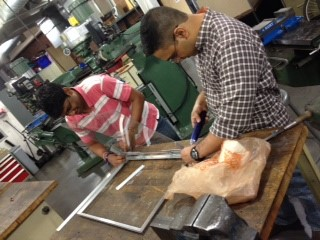
\includegraphics[width=2.5in]{p5.png}
						\caption{Structure Design.}
						\end{center}
						\end{figure}
						
						There are certain procedures that we followed in order to construct our holography display case as close as possible to our design. In order to build the structure of our hardware we used materials such as an Acrylic glass, two big metal (aluminum) bar, a ruler along with screw drivers and other small and big tools used to model the structure of our holography display case. This process is explained in the following steps:\newline
					
						\begin{figure}[htb]
						\begin{center}
						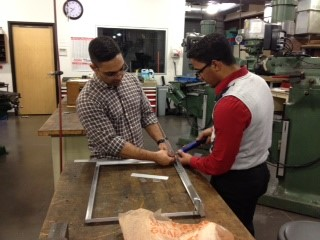
\includegraphics[width=2.5in]{p6.png}
						\caption{Structure Design.}
						\end{center}
						\end{figure}
						
						We first built the frame, or base, of our hardware. We did this by cutting the front and back of the frame in approximately 25 inches. Then, we proceeded to cut the sides in approximately 30 inches. Once we had the frame done, we proceeded to place two hinges on each corner of the frame to hold the frame. Our efficient manner of installing the hinges allows one to display the holographic 3D game in the angle of your preference. Also, we built a medal support so the glass does not bend while opening or closing the case. Lastly, we used the Leap Motion device as the hardware to interact with our computer. This gives the user the feeling that you are directly interacting with the game in a real environment. The reason for this is because you are moving your hands to play instead of a remote control.\newline
					
						\begin{figure}[htb]
						\begin{center}
						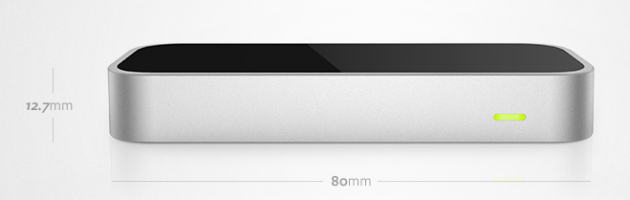
\includegraphics[width=2.5in]{p7.png}
						\caption{Structure Design.}
						\end{center}
						\end{figure}
												
						The Leap Motion controller is a USB peripheral device, which we plugged facing upward into our laptop. It uses two monochromatic infrared cameras and three infrared LEDs to observe a distance of about 3 feet in a semi hemispherical manner. In fact, the camera generates 300 frames per second of reflected data and sends this to the controller to be analyzed. As you can see in figure 10, the Leap Motion Controller is a sleek, light, and tiny device that is 3″ long. You can tell from the image, the Leap Motion hardly took up any space on our desk since we only used the space above it.
						\newline  
					} 
		
					\item {Performance} {\normalfont\newline 
						Screw drivers, tape measurement and other tools were very helpful to speed up and make our hardware construction possible. It was of great help to have available the workshop at RIT. It helped us avoid hard manual labor such as cutting the medal and modeling our own frame to build the base support for the glass.
					\newline
					}	
			\end{itemize}}}
	\end{enumerate}}

\section{Implementation}
\label{implementation}
	The Implementation section describes how our program applications will be installed, deployed, and transitioned into our operational system for the purpose of our project. In this section we will give an overview of the system, describe major tasks involved in the implementation process, and the overall resources needed to support the implementation effort such as hardware, software, techniques, and other tools. Furthermore, we will present users with the documentation and tools necessary to make an informed decision on how to deploy our project to have a holographic projection of a 3D Pong game, or any other 3D game. In addition, multiple features have not been added and we will explain how they will be added and utilized in our project for a better implementation process. 
	
	{\bf \begin{enumerate}
				\item {Software and Hardware} {\normalfont\newline 
	
					\bf{\begin{itemize}
						\item {Appearance} {\normalfont\newline
							\begin{figure}[htb]
								\begin{center}
								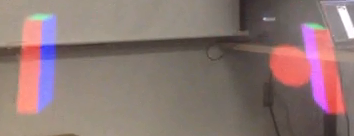
\includegraphics[width=1.0in]{p8.png}
								\caption{Structure Design.}
								
								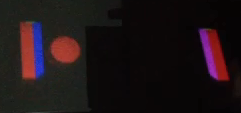
\includegraphics[width=1.0in]{p9.png}
								\caption{Structure Design.}
								
								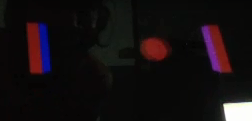
\includegraphics[width=1.0in]{p10.png}
								\caption{Structure Design.}								
								\end{center}
							\end{figure}
							
							Once we put the hardware and software together, the appearance of our holographic 3D game display can be seen in figures 11, 12, and 13. As you can see, the appearance of the holographic image highly depends on the lighting. We tested different scenarios to see which one gave a more realistic feeling of having real 3D objects in our environment.
						\newline
						}
			
						\item {Structure} {\normalfont\newline 
							\begin{figure}[htb]
								\begin{center}
									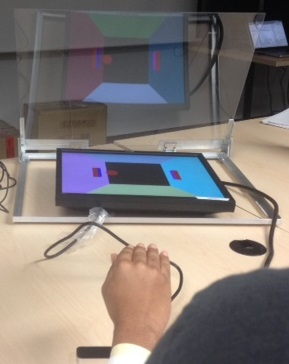
\includegraphics[width=1.5in]{p11.png}
									\caption{Structure Design.}
								\end{center}
							\end{figure}
							
							The image in figure 14 is how our setup looked once we put the software and hardware together, as per our design. Since our case did not have the box we planned it to have in order to stand, we have used a table as stand to hold the projector while it displayed the 3D game.\newline
						
							As you can see in the image in figure 14, the projector displayed the game through the flat monitor after we inserted our case. Then, once the game started we played through the leap motion, as shown in figure  14. \newline
						
							In order to successfully implement our project, we first placed the monitor on the desk. Then, we started the game on the laptop and connected the flat screen to the laptop. Afterwards, we adjusted the glass to an angle of 85 degree so the image looks as if it was right in front of our eyes. Finally, we adjusted the lighting of the room to start playing in different scenarios, as shown in figures 15, 16, and 17. 
						\newline  
						} 
			
						\item {Performance} {\normalfont\newline 
							\begin{figure}[htb]
								\begin{center}
									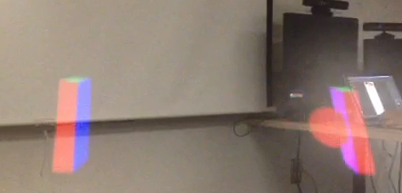
\includegraphics[width=2.0in]{p12.png}
									\caption{Structure Design.}
															
									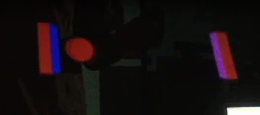
\includegraphics[width=2.0in]{p13.png}
									\caption{Structure Design.}
															
									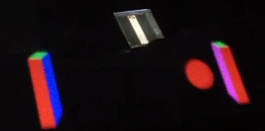
\includegraphics[width=2.0in]{p14.png}
									\caption{Structure Design.}								
								\end{center}
							\end{figure}
														
							The three images you see in figures 15, 16, and 17 are three of the best scenarios in which our project implementation was performed at its best. As you can observe, the image in figure 14 has a more real object environment feeling than the others. It looks as if the objects were real and they were floating in the air. However, you cannot see its surrounding and that takes out the purpose of our project. In the image in figure 12, you can clearly see its surrounding but the images are somewhat transparent. In this case, you can see through the images and is not clear that the objects are real. In the image in figure 13, you can partially see the surrounding and you are also able to see the objects as if they were real. This was, from our perspective, the best scenario derived during our implementation. 
						\newline
						}	
				\end{itemize}}}
		\end{enumerate}}
	
\section{Current Work}
\label{current work}
	The current status of our project is being explained through the two main sections that highly influenced the development of our project. These two main sections are the Software and Hardware implementation, and their development process is explained in the following manner.\newline 
	
	\subsection{Software}
	
		Goal and Achievements\newline
	
		In this section, our goal was to create an entertaining game that can easily allow the user to interact with its components. For this project, we chose a 3D Pong game since this, along with the Leap Motion, would allow users to interact with the pads as if they were holding it. A holographic display of this image would give users a real environment feeling.\newline

		We were able to create almost the entire scenario of the 3D Pong game. We have developed the game in 2D, which we could have easily added to our implementation. We did not add it because our game is devoid of the physics component. Therefore, it would make no sense including the 2D game since no player would win.\newline
		
	\subsection{Hardware}
	
		Goal and Achievements\newline
		
		In this section, our goal was to create our own holography display case to project the 3D Pong game. We wanted the game to look as if the user was playing it in real environment, and not on the computer. For this, we made use of the Leap Motion device to make the interaction of the user and game more realistic.  \newline
		
		On the other hand, we were able to create the entire frame of our holography display case. In fact, we made the case adjustable to project the holographic images in different angles. \newline
	
\section{Future Work}
\label{future work}
	\bf{\begin{itemize}
					\item {Software} {\normalfont\newline
						Physics Simulation\newline
						
						In order for the 3D Pong game to have a realistic feel, it is imperative to simulate real world physics as best as possible. As an improvement to our interface, the system needs to calculate forces, speed and acceleration based on a simulated mass. This is required along with calculations for collisions and collision detection. \newline
						
						The goal is to have the balls position step back once a collision is detected between the ball and the paddle. Afterwards, the ball must have its speed and direction modified based on where the paddle hits. Initially, this will imply having the paddles not shift in the depth (x, z) plane and only the height-width plane (x, y) to replicate pongs paddle up-down movement. In particular resolving the collision ball-paddle is reduced to resolving the collision of a ball against a wall. This idea similar to our implementation is found on [1], which discusses how physics should be applied in a 3D environment. This goes through the equations required to correctly simulate rotational physics on a computer generated environment based on a billiards game.
						\newline
	 				}
	 				\item {Hardware} {\normalfont\newline
	 					The holography display case that we built was almost complete according to our design. The only work that completely matched our design was to create a box to work as the base of the frame. This way, we would be able to use it as a stand while holding the projector to display the holographic 3D game. Also, we could make this case have a more sleek design. In order to achieve this look, our hardware would resemble a small business brief case that we could easily carry around, lock, and unlock when needed.
						\newline 
					}
			\end{itemize}}


\section{Conclusion}
\label{conclusion}\normalfont 
		This project named, “Holographic Pong,” was prepared in response to a more stimulating and innovating entertainment environment in which users sustain a more interactive feel while playing their game. The full implementation of our project, over the coming years, will ensure users to have the observational information needed to understand how to display a holographic projection of a 3D Pong game or any other 3D game. The 3D feel is amplified when one takes the image projected from one location to another location where the hologram is projected in real-time as a 3D display. Our project could easily be pertinent to the entertainment arena, where such technology is being utilized in the industry. This project is also a representation of what new and exciting applications are on the horizon and with only a few modifications and improvements, can be incorporated into the functional realm of our daily lives. It will address the commitments of the users to change the way they have always played games in the past.  \newline
		
		There are sustained annotations of the essential techniques that are used to make significant progress in this generation of 3D gaming as well as other derived information for our project. These annotations give an enhanced support to our research, modeling, and analysis to build a holographic 3D game. In fact, these interpretations could highly improve and add important features into our project. Other observations, described in Future Work, must be sustained into the future to evaluate new technology and improve our project implementation for a better 3D Pong game holographic projection. It is crucial for users to base any implementation of this project on the supported given material as well as the research needed, which can easily refine the holographic projection. \newline 
	
\bibliographystyle{abbrv}
\bibliography{report}
% You must have a proper ".bib" file
%  and remember to run:
% latex bibtex latex latex
% to resolve all references
%\balance

\end{document}